\documentclass[12pt, a4paper, oneside]{article}
%die Pakete werden hier durch den Include-Befehl separat eingelesen
\usepackage[utf8]{inputenc}
\usepackage{amsmath} % Mathematik-Pakete
\usepackage{amsfonts}
%\usepackage{mathptmx} %times new roman
%\usepackage[T1]{fontenc} %vollen Zeichensatz ]
\usepackage{amssymb}
\usepackage[ngerman]{babel}
\usepackage{graphicx}
\usepackage{microtype} %besserer Randausgleich
\usepackage{footnote}
\usepackage{blindtext}
\usepackage{etoolbox}
%\usepackage{makeidx}
%\usepackage{dsfont}
\usepackage{lettrine}%\usepackage{geometry}
%\usepackage{xcolor} % Für verschiedene Farben
\newcommand{\ricardo}[1]{\colorbox{ForestGreen}{\color{white}   \textsf{\textbf{Ricardo}}} \textcolor{ForestGreen}{#1}}
\usepackage[pdfborderstyle={/S/U/W 1}]{hyperref} % Für interaktive Refernzierung im PDF
\usepackage{csquotes}
\usepackage{acro}
\usepackage{hyperref} % Für interaktive Refernzierung im PDF
\usepackage[onehalfspacing]{setspace}%Zeilenabstand 1.5
% \usepackage{picins} % Das Umfließen einer Grafik im Text kann mit dem Paket PicIns erreicht werden.
%\usepackage{fontspec} 

%\usepackage[utf8]{inputenc}
\usepackage[ngerman]{babel}
\usepackage[top=2.5cm, bottom=2.5cm, left=2cm, right=3.5cm]{geometry}
\usepackage{bibgerm}
\usepackage{tabularx}
\usepackage{adjustbox}
\usepackage{cite}
\usepackage{blindtext}
\usepackage{epsfig}
\usepackage{longtable}
%\usepackage{showframe}
\usepackage{dcolumn}%benötigt für stargaze
\usepackage{here}%lädt das Paket zum Erzwinge n der Grafikposition
\usepackage{floatflt}%Bilder im Fließtext
%\usepackage{fontspec}
%\usepackage{fontenc}
\usepackage{dsfont}
%\setsansfont[Ligatures=TeX]{Arial}
%\renewcommand{\familydefault}{\sfdefault}
%\usepackage{times}
\usepackage{graphicx}
\usepackage{epstopdf}

\usepackage{xcolor}
\usepackage{listings}

\usepackage{lipsum}




\lstset{language=R}
\lstset{basicstyle=\ttfamily,
basicstyle=\small}
\lstset{literate=%
  {Ö}{{\"O}}1
  {Ä}{{\"A}}1
  {Ü}{{\"U}}1
  {ß}{{\ss}}1
  {ü}{{\"u}}1
  {ä}{{\"a}}1
  {ö}{{\"o}}1
}

\title{\textbf{Projektdokumentation eFinder}}
\author{Lukas Räpple \& Etienne Gotha}

\setlength{\parindent}{0cm} %keine Einrückung
\linespread{1.5} 
\acsetup{first-style=short}
\newpage


\newpage
%in alphabetischer Reihenfolge

\newcounter{SeitenzahlSpeicher}
\begin{document}

 \thispagestyle{empty}
\begin{titlepage}
	 \thispagestyle{empty}
	% thispagestyle{empty} unterdrückt Seitenzahlen auf der gewünschten Seite
	\newfont{\smc}{cmcsc10 at 12pt}
%	\maketitle
	%Aufpassen mit fi: Fehlercode U+FB01
	%%%%%%%%%%%%%%%%%%%%%%%%%%%%%%%%%%%%%%%%%%
%Titel, Autor, Seminar, Semester, Dozent %
%%%%%%%%%%%%%%%%%%%%%%%%%%%%%%%%%%%%%%%%%%
\begin{center}
	 \thispagestyle{empty}
\begin{figure}[t]
	\centering
	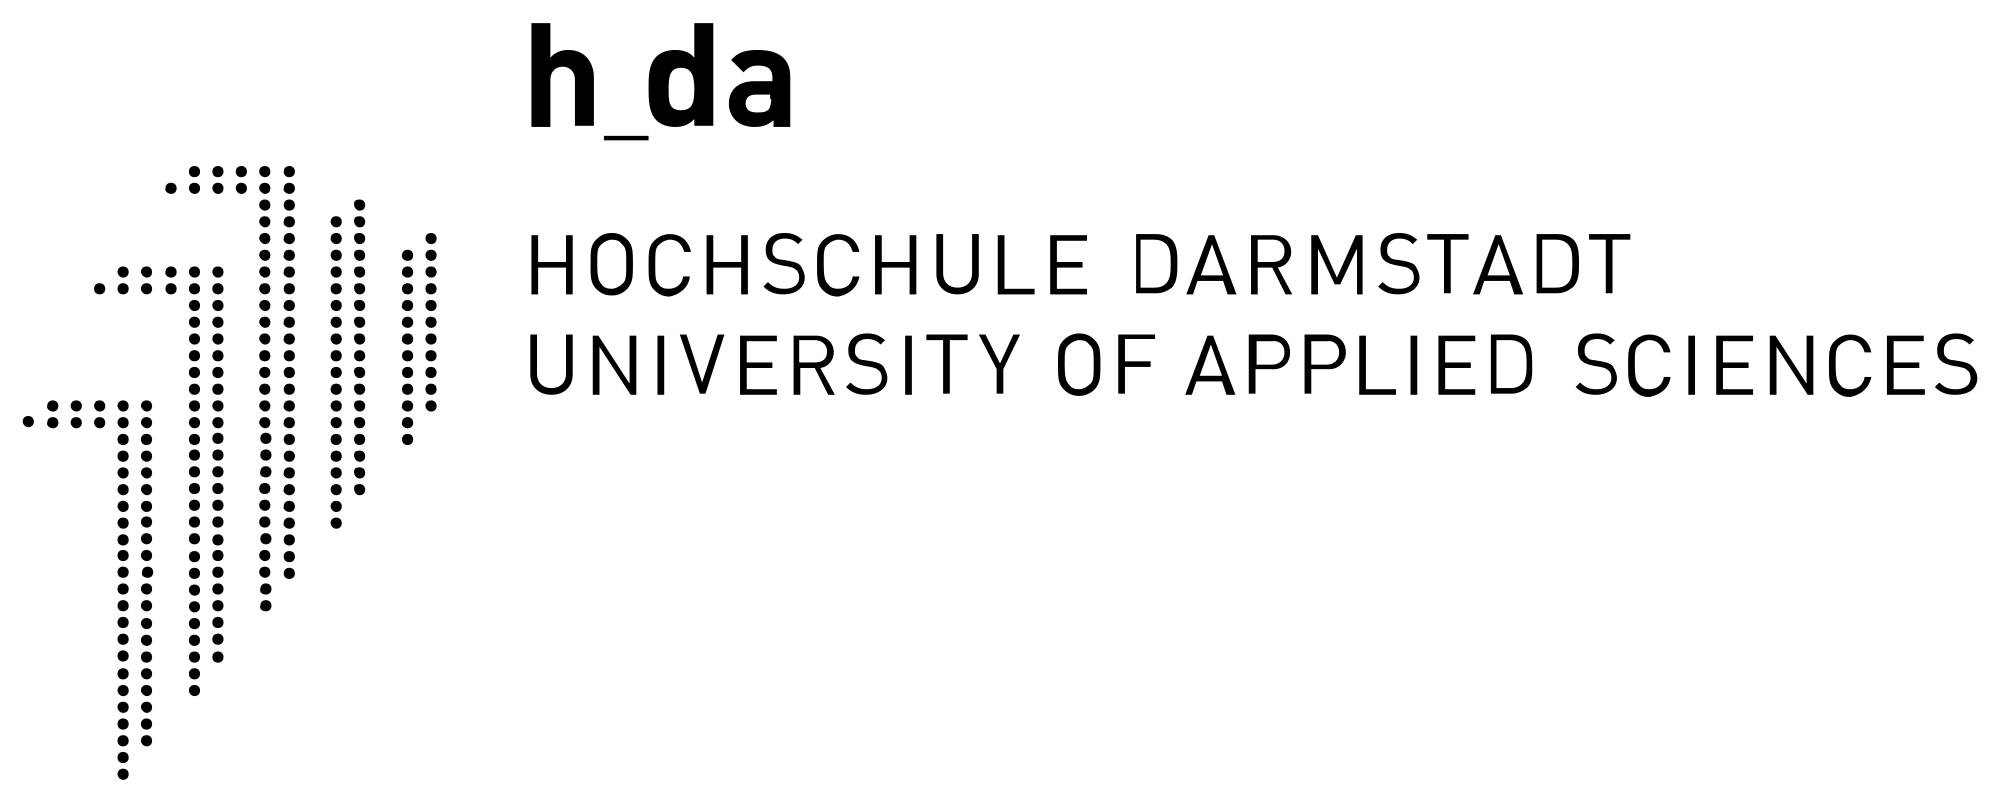
\includegraphics[width=0.6\textwidth]{Hda_logo.svg.png}
	
\end{figure}

$~~$\\
\paragraph{}$~~$\\
\paragraph{}$~~$\\
\textbf{\huge Projektdokumentation eFinder}\paragraph{}$~~$\\
\paragraph{}$~~$\\
\paragraph{}$~~$\\
\textbf{im Rahmen des Fachs Nutzerzentrierte Softwareentwicklung}\\ \textbf{am Fachbereich Informatik}\\ \textbf{der Hochschule Darmstadt}
\paragraph{}$~~$\\
\paragraph{}$~~$\\
\paragraph{}$~~$\\
\paragraph{}$~~$\\
\text{von: Lukas Räpple \& Etienne Gotha}\\
\text{Dozent: Prof. Dr. Hans-Peter Wiedling}\\
\end{center}	
\end{titlepage}



\begin{spacing}{1}
\pagenumbering{Roman}
\setcounter{page}{2}
\tableofcontents
\end{spacing}
\newpage
\begin{spacing}{1}
\section*{Abbildungsverzeichnis} 
\addcontentsline{toc}{section}{Abbildungsverzeichnis}
\renewcommand{\listfigurename}{}
\listoffigures
\end{spacing}
\newpage
\clearpage
\setcounter{SeitenzahlSpeicher}{\value{page}}
\pagenumbering{arabic}
\newpage
\pagenumbering{arabic}

\section{Einführung}
Das vorliegende Projekt entstand im Rahmen des Praktikums zur Veranstaltung Nutzerzentrierte Softwareentwicklung im Wintersemester 2021/2022 an der Hochschule Darmstadt. Im Folgenden wird der Ablauf des Projektes von der Konzeption bis zur Auswertung der Ergebnisse dargestellt.

\subsection{Projektbeschreibung}
Gegenstand des Projektes ist die Entwicklung einer prototypischen Anwendung, die verschiedenen Nutzern den Zugang zu Informationen und Diensten bezüglich Ladestationen für Elektrofahrzeuge bereitstellt. Als Entwicklungsplattform wird Android Studio mit der Programmiersprache Java verwendet. Die Applikation soll sich dabei gleichermaßen an Fahrer von Elektrofahrzeugen als auch an Servicekräfte/Techniker, die für den Betrieb der Ladestationen zuständig sind, richten. Ziel des Projektes ist es einen durchgehend auf diese Nutzergruppen ausgerichteten Entwicklungsprozess zu durchlaufen, um ein möglichst hohes Maß an Usability zu erreichen.

\subsection{Vorgehensweise}
Die Durchführung des Projektes und somit auch der vorliegenden Dokumentation orientiert sich am Wasserfallmodel. Das Model kann in die fünf Phasen Analyse, Design, Implementierung, Test und Betrieb unterteilt werden \cite[S. 16 ff.]{SoftwareDevelopmentBestPractices}. Da es sich beim vorliegenden Projekt um die Erstellung eines Prototypen handelt, wird allerdings auf eine Betrachtung der Phase Betrieb verzichtet.\\

Im ersten Schritt des Projektes wird eine heuristische Anforderungsanalyse durchgeführt. Dabei werden begründete Annahmen darüber getroffen, in welchem Kontext die Anwendung vermutlich verwendet wird und welche Intentionen beziehungsweiße Anforderungen die einzelnen Nutzergruppen mit sich bringen.\\

Die darauf folgende Designphase befasst sich zunächst mit den Fragen, wer der durchschnittliche Benutzer ist und welche Ziele er mit der Benutzung der Anwendung verfolgt. Dafür wird einerseits ein durchschnittliches Nutzerprofil in Form einer Persona für jeweils den Elektroautofahrer und den Servicemitarbeiter erstellt. Außerdem werden User Stories zu den beiden Nutzergruppen verfasst, die in Form von kurzen Statements Bedürfnisse darlegen, die der Nutzer mit der Anwendung befriedigen möchte. Auf Basis dieser Ergebnisse wird dann ein Paper Prototyp erstellt, der den Aufbau der einzelnen Ansichten/Screens skizziert.\\

Für die Implementierung des zuvor erstellten Designs werden im ersten Schritt Überlegungen zum Aufbau der Software und der Kopplung einzelner Funktionalitäten aufgestellt. Danach wird die Anwendung agil entwickelt, indem möglichst früh ein fertiges Produkt geliefert wird. Dieses Produkt wird dann im Rahmen des vorhandenen Zeithorizonts iterativ durch weitere Komponenten ergänzt. Zur Verwaltung des kooperativ erstellten Codes wird ein Git Repositorium verwendet, wo die einzelnen Sprints als Issues angelegt sind.\\

In der letzten Phase des Projektes wird die Anwendung hinsichtlich ihrer Funktionalität und Usability getestet und bewertet.\\

\section{Analyse}
\subsection{Heuristische Anforderungsanalyse}
Betrachten wir zunächst die Umstände, die den Fahrer eines Elektroautos dazu verleiten könnten eine App für Ladestationen zu nutzen. Eine Intention, die als häufiger Kontext für die Verwendung der App angenommen werden kann, ist die Suche nach einer Ladestation in der näheren Umgebung des Nutzer. Eine leere Batterie, eventuell noch in einer unbekannten Umgebung, sind wieder auftretende Situationen, die eine schnelles Auffinden der nächsten Ladesäule nötig machen.\\

Am 01.01.2022 sind im Bundesgebiet 44.486 Ladesäulen gemeldet. Damit ist die Auswahl an Ladestationen in einem Jahr um 10.048 gestiegen. Allerdings ist der Ausbau der Infrastruktur im Vergleich der Bundesländer und vor allem im Vergleich zwischen Stadt und Land ungleich verteilt \cite[]{Ladeinfrastruktur2022}. Diese inkonsistente Netzabdeckung bringt Unsicherheiten für den Fahrer eines Elektroautos mit sich. Somit wird ein potentieller Nutzer von der App außerdem erwarten, dass er sich die Ladesäulendichte in einem weiter entfernten Reiseziel anzeigen lassen kann.\\

Desweiteren gibt es bei den einzelnen Ladesäulen deutliche Unterschiede. Einerseits hinsichtlich des Preises und andererseits hinsichtlich angebotener Steckertypen und Ladegeschwindigkeit. Aus der wachsenden Anzahl an Optionen eine informierte Entscheidung treffen zu können, ist somit ein weiterer Anreiz für die Verwendung der App. Die Verschiedenheit der Ladesäulen und ihre relative Entfernung zum Wohnort des Nutzers führen unausweichlich dazu, dass einzelne Ladesäulen regelmäßig aufgesucht werden. Die präferierten Ladesäulen sollten daher vom Nutzer schnell aufgerufen werden können.\\

Eine relevante Information für einen Fahrer ist außerdem die momentane Verfügbarkeit einer Ladesäule. Das Aufladen eines E-Autos dauert deutlich länger als etwa die Tankdauer eines Autos mit Verbrennungsmotor. Der Ladevorgang bei einer herkömmlichen öffentlichen Ladesäulen dauert etwa 2 bis 4 Stunden und bei einer Schnellladesäulen immer noch 0.5 bis 1 Stunde \cite[]{Ladedauer}. Ein Nutzer hat somit ein Interesse daran zu wissen, ob die Ladesäule gerade besetzt ist oder nicht.\\

Servicemitarbeiter/Techniker benötigen die App dagegen im Kontext ihres Anstellungsverhältnisses. Sie sind für die Reparatur und Wartung der Ladesäulen zuständig. Dafür müssen Sie einerseits ebenfalls den Standort einer Ladesäule einsehen können und andererseits wissen, welche Ladesäulen einen Defekt aufweisen. Daher wird ein Techniker erwarten, dass ein Kunde ein Problem mit einer Ladesäule melden kann und eine Liste dieser Meldungen für den Mitarbeiter ersichtlich ist.\\

Während jeder Kunde in der Lage sein sollte defekte Ladesäulen zu melden, sollte eine Reparatur nur von einem dafür dedizierten Mitarbeiter gemeldet werden können. Dafür sollte es einen abgetrennten Bereich in der Anwendung geben, der nur für Anwender mit bestimmten Administratorrechten zugänglich ist.\\

\section{Design}
\subsection{User Story Mapping}
\subsection{Persona}
\subsection{Paper-Prototyping}

\section{Implementierung}
\subsection{Softwaredesign}
\subsubsection{Klassen \& Kopplung}
\subsection{Umsetzung der Screens und Funktionalitäten}
\subsubsection{Datenbankintegration}
Damit die Daten der Applikation persistent gemacht werden können und nicht bei jedem Abschalten der Anwendung verloren gehen, wird eine Datenbank mithilfe der Plattform Firebase angelegt. Dabei wird einerseits die dedizierte Authentifizierungsfunktionalität und andererseits die bereitgestellte NoSQL-Realtimedatabase verwendet. Die Datenbank kann über den integrierten Firebase Assistenten in Android Studio unter Verwendung des API-Schlüssels mit der App verbunden werden. So kann man sich über den Aufruf der Funktion getInstance eine Referenz zur vorhanden Datenbankinstanz für den Authentifizierungsbereich und der Realtime Database holen(Abbildung 1). Wie die einzelnen Daten darin gespeichert werden, wird im weiteren Verlauf dargestellt.\\
\newpage
\begin{figure}
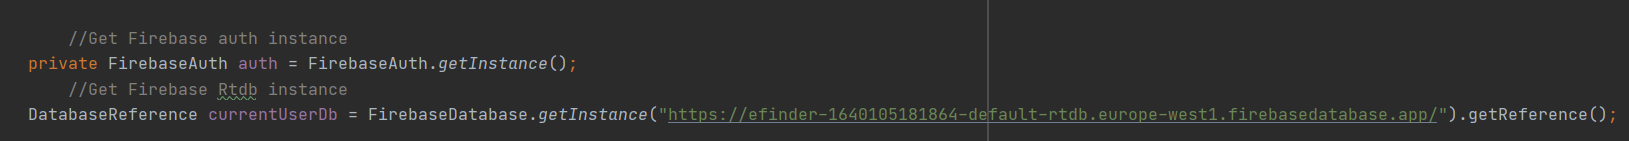
\includegraphics[width=1\textwidth, height=2cm]{firebase_connect.png}
\centering
\label{input_check}
\caption{Generierung der Datenbankreferenzen}
\end{figure}
\subsubsection{Registrierung \& Login}
Beim erstmaligen Öffnen der App wird der Nutzer zum Login-Screen(Abbildung 2) weitergeleitet.  Beim Aufruf der Login-Activity wird zunächst durch das Aufrufen der Funktion isLoggedIn überprüft, ob bereits eine Authentifizierungsinstanz existiert und wenn ja, wird der Nutzer direkt zur Main-Activity weitergeleitet(Abbildung 3).\\

Wenn bereits ein Konto existiert, aber keine offene Authentifizierungsinstanz gefunden wurde, kann der Nutzer sich mit seiner E-Mail und Passwort anmelden. Nach drücken des Buttons mit dem Label "`Login'' wird die Funktion authenticateUser aufgerufen, die mit Hilfe der von Firebase bereitgestellte Funktion signInWithEmailAndPassword überprüft, ob die eingegebene E-Mail und das eingegebene Passwort korrekt sind(Abbildung 4). Erst dann wird der Nutzer zur Main-Activity weitergeleitet.\\ 

\begin{figure}
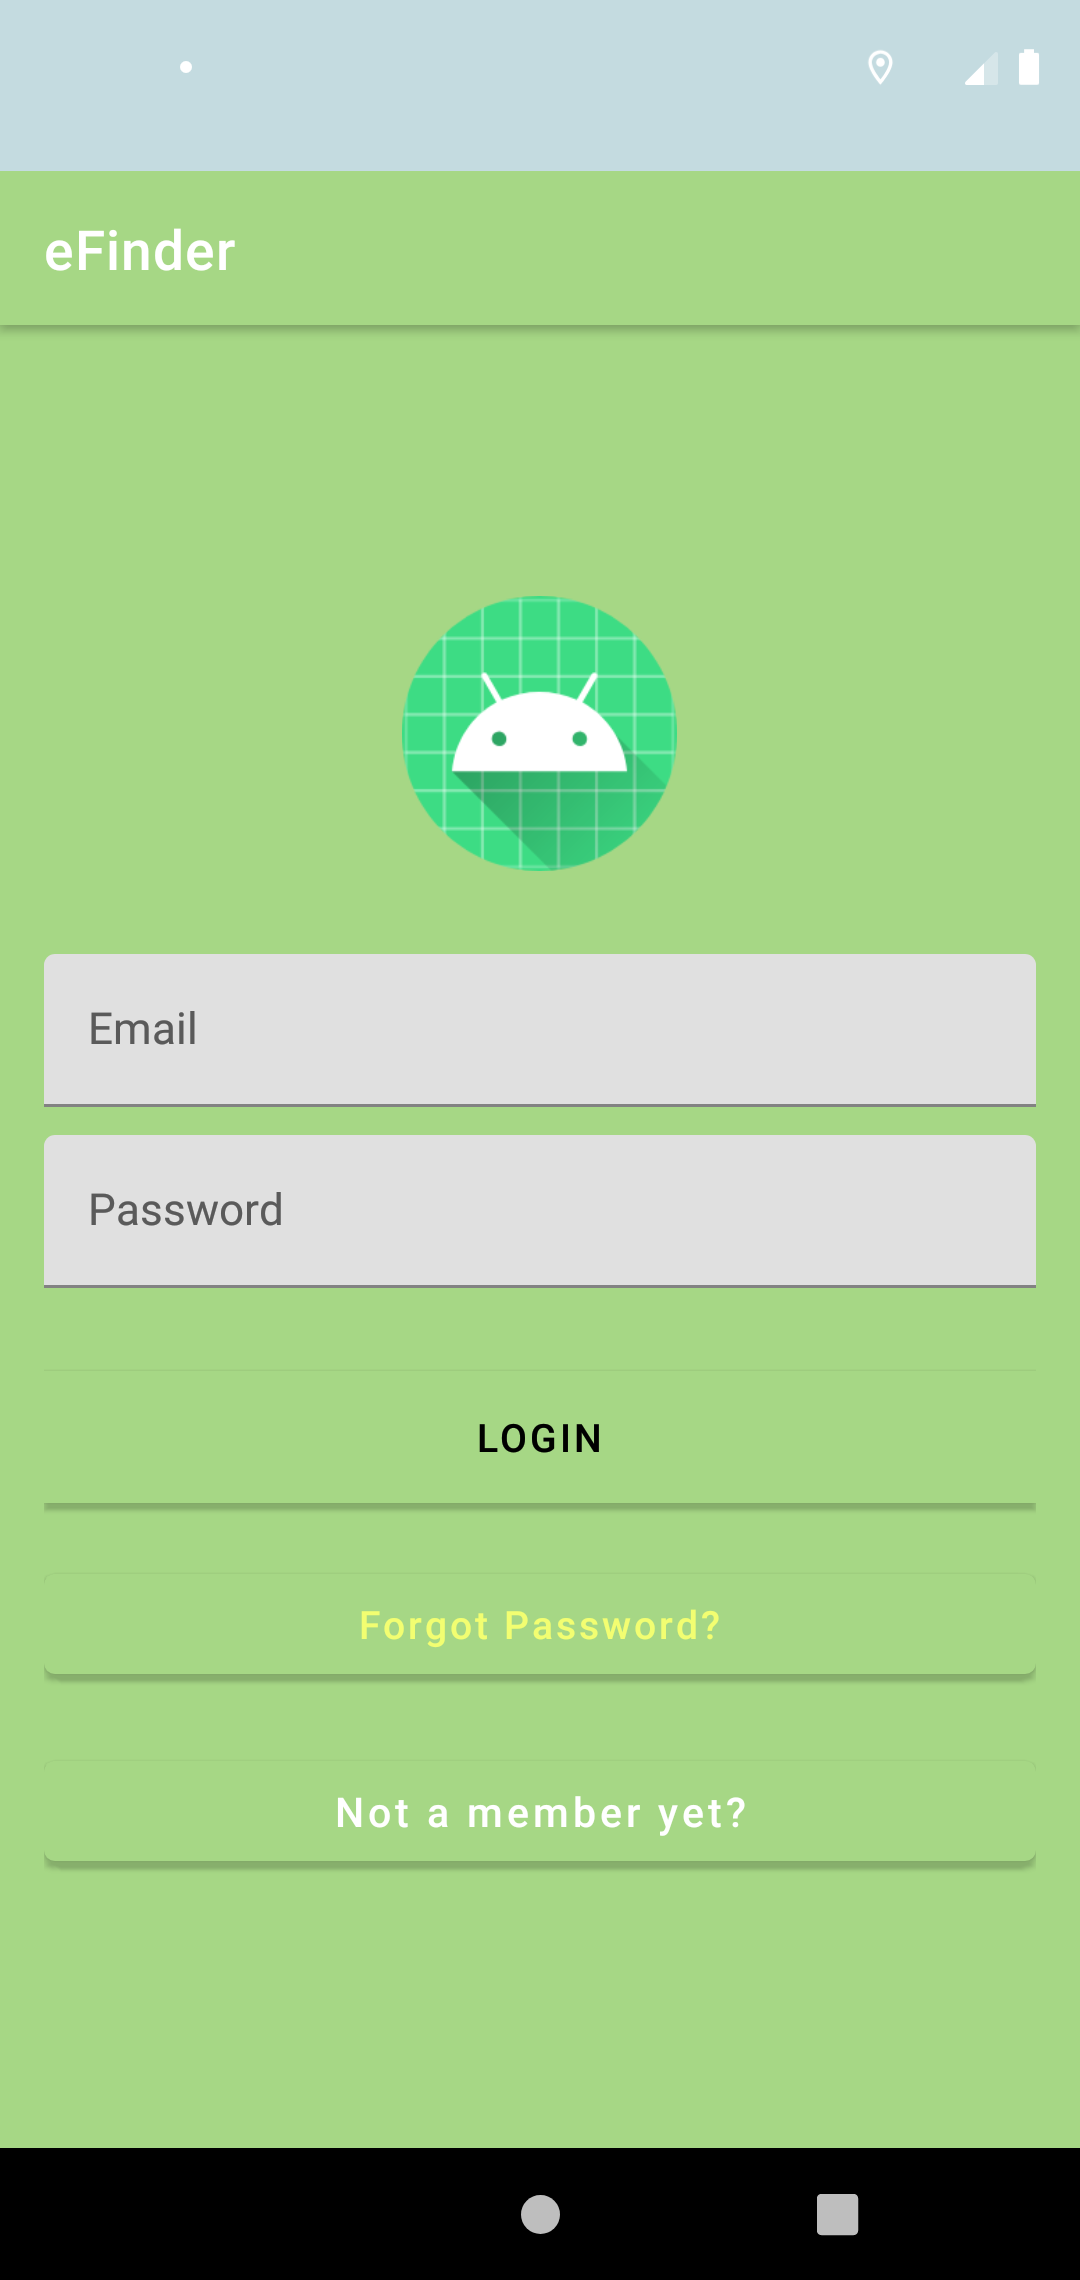
\includegraphics[width=5cm, height=9cm]{Login-Screen.png}
\centering
\label{login}
\caption{Login-Screen}
\end{figure}
\begin{figure}
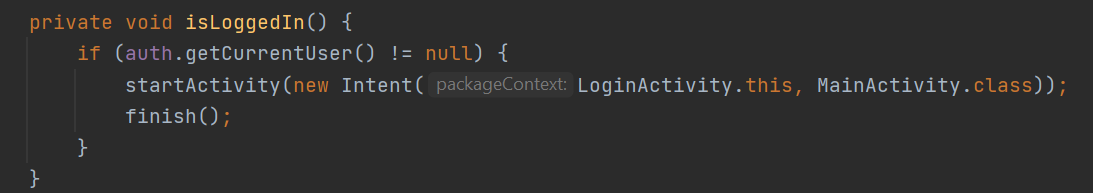
\includegraphics[width=1\textwidth, height=3cm]{isLoggedIn.png}
\centering
\label{isLoggedIn}
\caption{Abfrage der existierenden Authentifizierungsinstanz}
\end{figure}
\begin{figure}
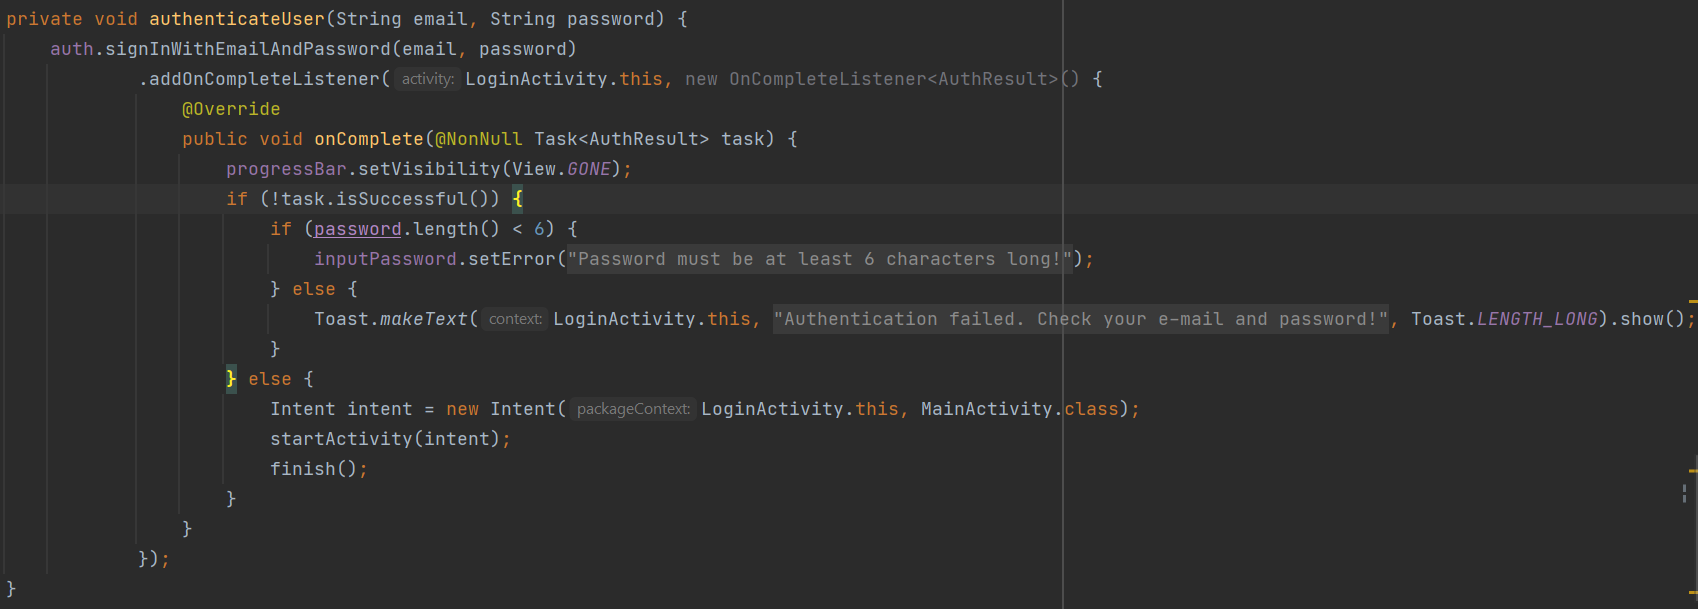
\includegraphics[width=1\textwidth, height=7cm]{authentication.png}
\centering
\label{authentication}
\caption{Authentifizierung des Benutzers}
\end{figure}
Hat der Nutzer noch keinen Benutzer angelegt, kann er sich über den Button mit der Beschriftung " `Not a member yet?'' zum Registrierungs-Screen(Abbildung 3) weiterleiten lassen. Wenn der Nutzer dort auf den Button mit der Beschriftung "`Login'' drückt, wird zunächst getestet, ob er die nötigen Information in die dafür vorgesehen EditText-Felder eingegeben hat und ob das Passwort eine Länge von mindestens 6 Zeichen aufweist. Ist dies nicht der Fall, wird der Nutzer darauf hingewiesen(Abbildung 4).\\

\begin{figure}
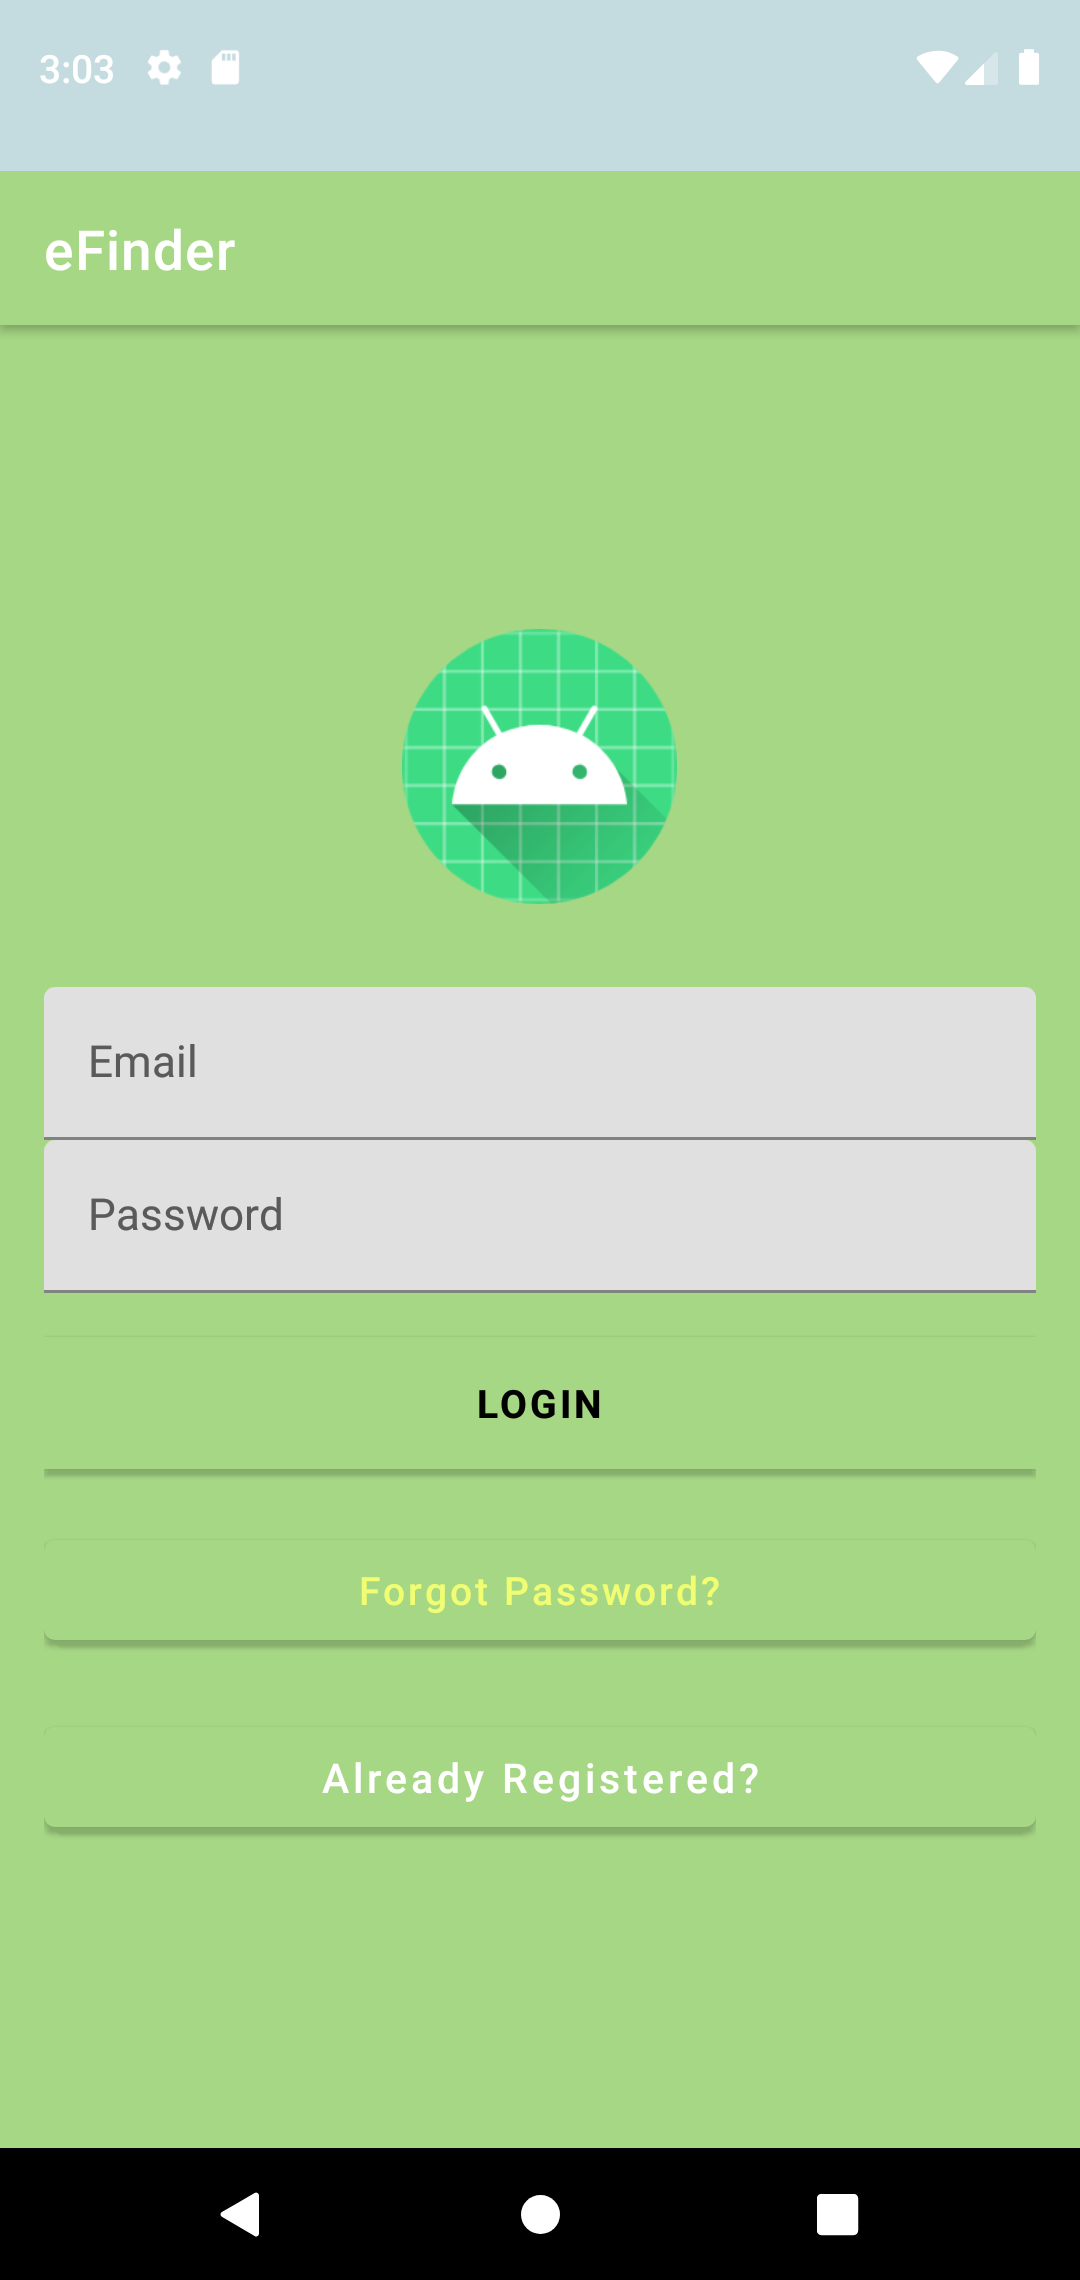
\includegraphics[width=5cm, height=9cm]{Registrierungs-Screen.png}
\centering
\label{register}
\caption{Registrierungs-Screen}
\end{figure}
\begin{figure}
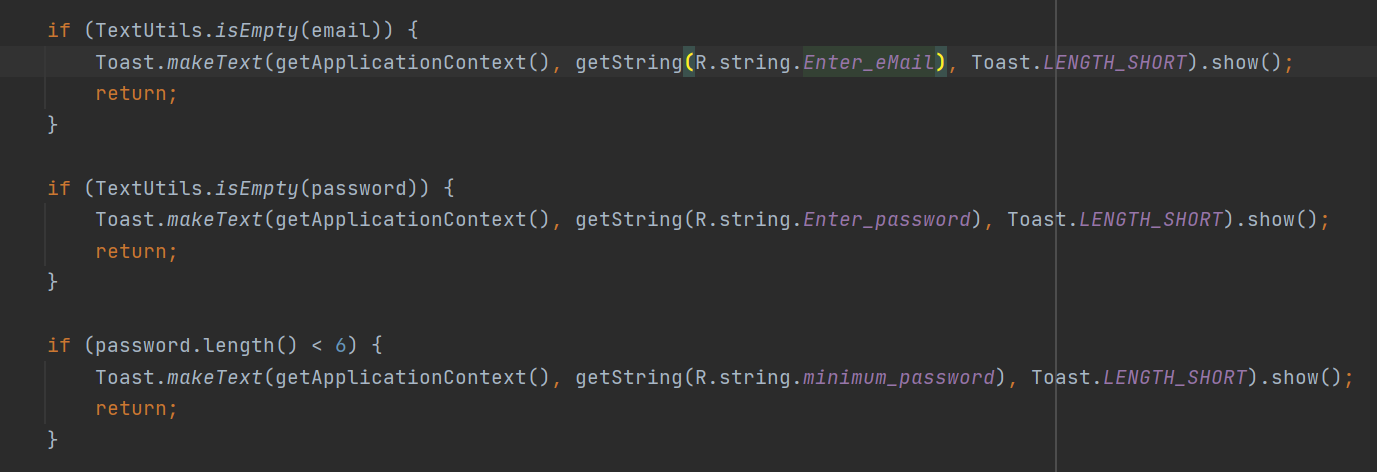
\includegraphics[width=1\textwidth, height=7cm]{SignUp_check.png}
\centering
\label{input_check}
\caption{Überprüfung des User-Input}
\end{figure}
Wurden alle Eingabevoraussetzung vom Nutzer erfüllt, wird durch das Aufrufen der Funktion saveNewUser ein neuer Benutzer in der Datenbank angelegt(Abbildung 5). Die Funktion createUserWithEmailAndPassword wird von Firebase bereitgestellt, um einen neuen Eintrag im Authentifizierungsbereich anzulegen(Abbildung 6). Gleichzeitig wird ein neues User-Objekt erstellt und als Node in der Realtime-Database unter der ID des Benutzers angelegt. Wie das am Ende aussieht, kann in der Abbildung 7 gesehen werden. Nach erfolgreicher Registrierung wird der Nutzer zur MainActivity weitergeleitet. 
\begin{figure}
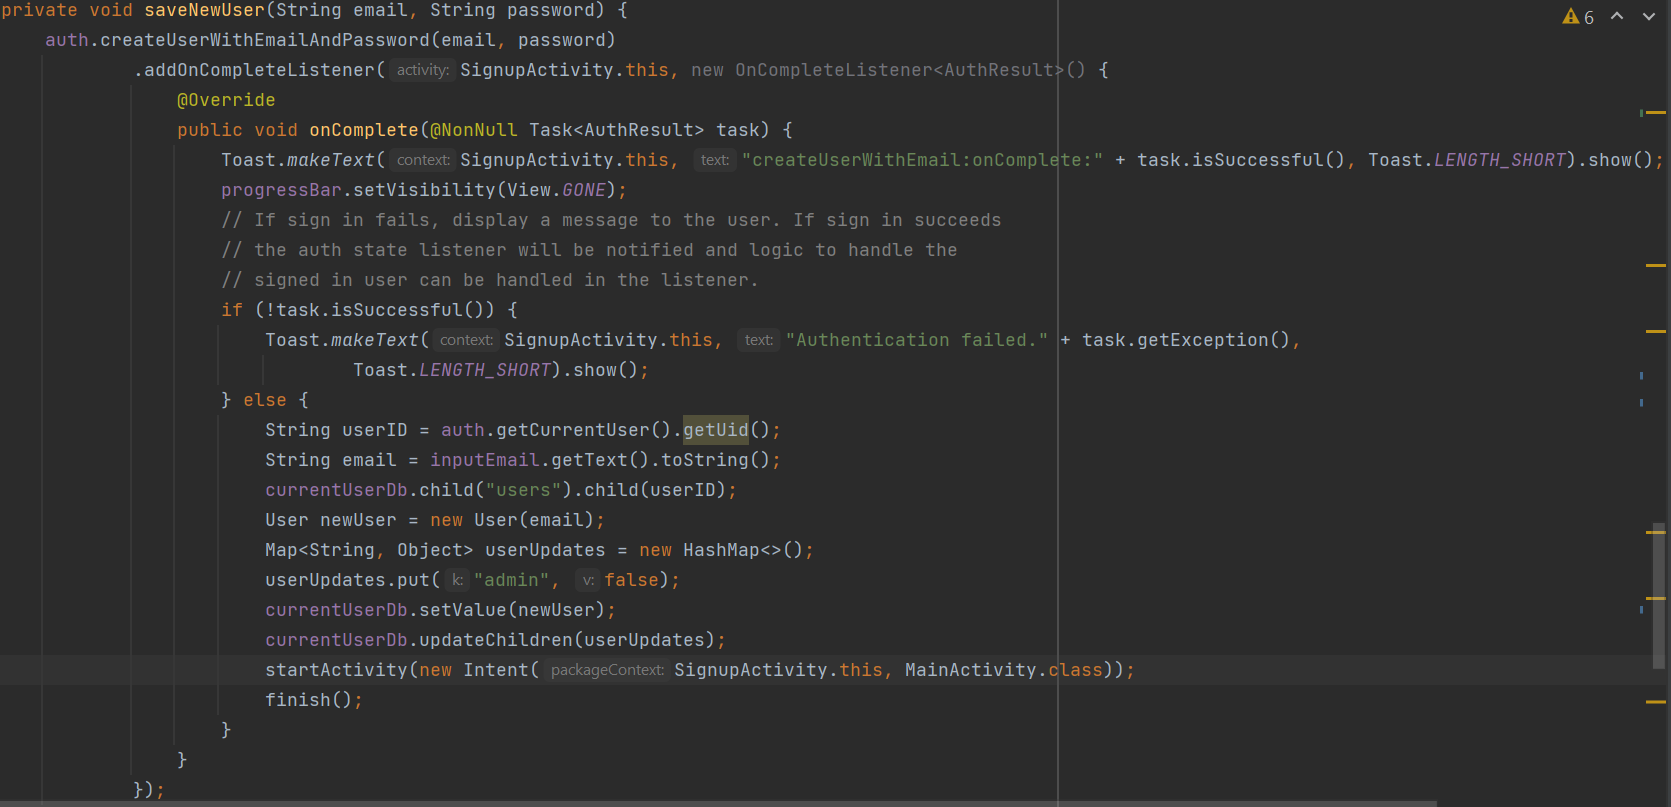
\includegraphics[width=1\textwidth, height=10cm]{save_user.png}
\centering
\label{new_user}
\caption{Anlegen eines neuen Benutzers}
\end{figure}
\begin{figure}
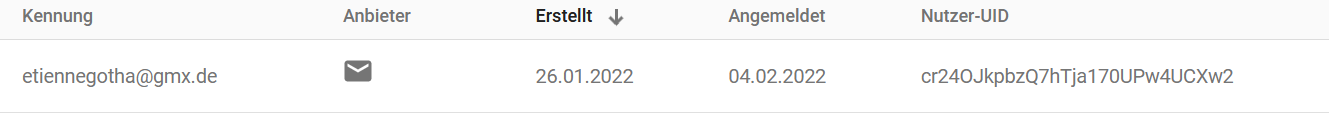
\includegraphics[width=1\textwidth, height=1.5cm]{User_In_Auth.png}
\centering
\label{auth_user}
\caption{Nutzer im Authentifizierungsbereich der Firebase}
\end{figure}
\begin{figure}
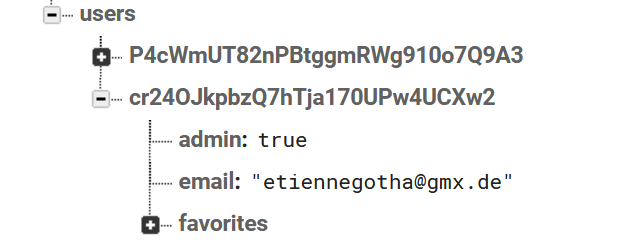
\includegraphics[width=0.5\textwidth, height=5.5cm]{User_Rtdb.png}
\centering
\label{user_rtdb}
\caption{Nutzer in der Realtime-Database}
\end{figure}
\subsubsection{Navigationsleiste}
Nachdem der Nutzer zur Main-Activity weitergeleitet wurde, befindet er sich zunächst auf dem Map-Screen. Von dort aus kann er sich mit Hilfe einer Navigationsleiste(Abbildung 10) frei zwischen verschiedenen Screens(Map, Suchen, Admin, Favoriten, Einstellungen) bewegen. Die Navigationsleiste wird in der Main-Activity initialisiert und dort mit den einzelnen Fragmenten, welche die Views für die verschiedenen Screens enthalten, verbunden(Abbildung 11). Das Layout der Navigationsleiste wird über ein von Android bereitgestelltes AppBarConfiguration-Objekt gebildet. Über ein NavController-Objekt wird die Navigation zwischen den Fragmenten durch ein Host-Fragment in der XML der Main-Activity(Abbildung 12) organisiert.
\begin{figure}

\includegraphics[width=6cm, height=1cm]{Navigationsleiste.png}
\centering
\label{navbar}
\caption{Navigationsleiste}
\end{figure}
\begin{figure}
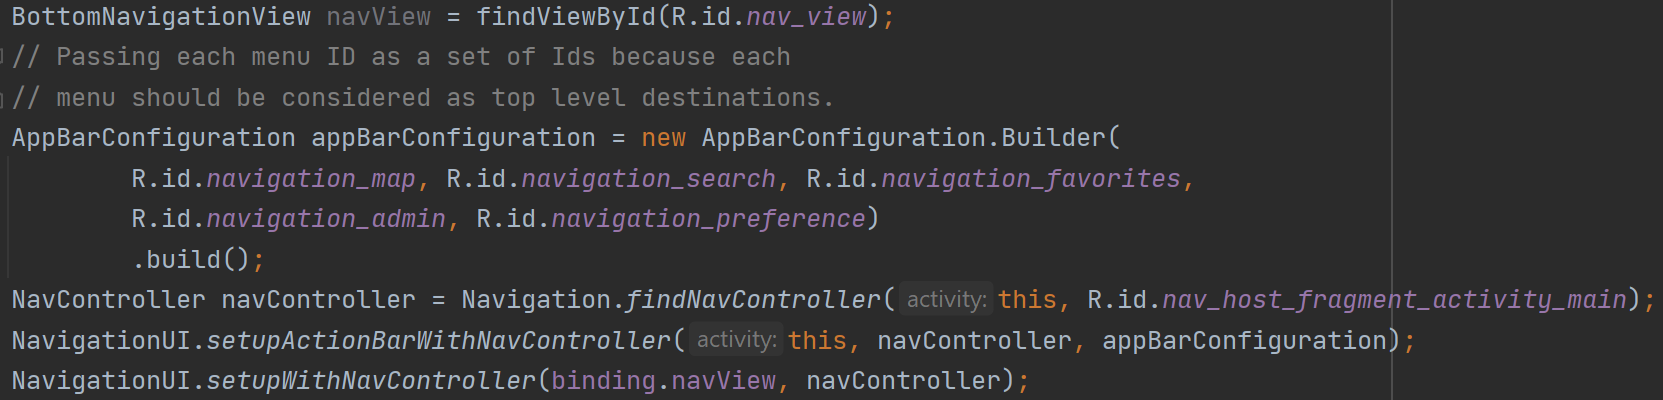
\includegraphics[width=1\textwidth, height=5.5cm]{navbar_setup.png}
\centering
\label{nav_setup}
\caption{Initialisierung der Navigationsleiste in der Main-Activity}
\end{figure}
\begin{figure}
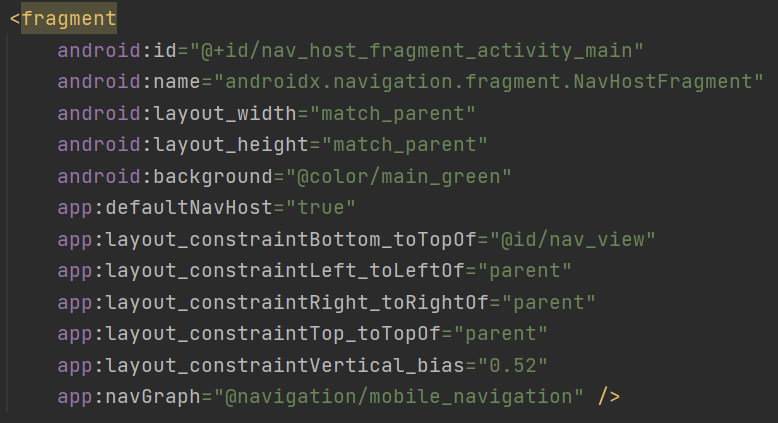
\includegraphics[width=0.8\textwidth, height=5.5cm]{Host-Fragment.png}
\centering
\label{host_fragment}
\caption{Host-Fragment in der XML der Main Activity}
\end{figure}
\subsubsection{Map-Screen}
\subsubsection{Suchen-Screen}
\subsubsection{Admin-Screen}
\subsubsection{Favoriten-Screen}
\subsubsection{Einstellungen-Screen}
\subsubsection{Mehrsprachigkeit \& Landscape-Mode}

\section{Test}
\subsection{Funktionale Tests}
\subsection{Usability-Test}
\newpage

\section{Fazit}

\section{Literaturverzeichnis}
\bibliographystyle{natdin}
\renewcommand{\refname}{} 
\bibliography{bibba}

\newpage


\appendix %Anhang
\pagenumbering{arabic}
\section{Anhang}

\newpage

\section{Eigenständigkeitserklärung}
``Ich versichere, dass ich die Arbeit selbständig und ohne Benutzung anderer als der angegebenen Hilfsmittel angefertigt habe. Alle Stellen, die wörtlich oder sinngemäß aus Veröffentlichungen oder anderen Quellen entnommen sind, sind als solche kenntlich gemacht. Die schriftliche und die elektronische Form der Arbeit stimmen überein. Ich stimme der Überprüfung der Arbeit durch eine Plagiatssoftware zu.''
\paragraph{}$~~$\\
\paragraph{}$~~$\\
\vspace{50pt} 
\noindent\rule{5cm}{.4pt}\hfill\rule{5cm}{.4pt}\par 
\noindent Ort, Datum \hfill Unterschrift 
\end{document}